\section{Transpose}
\label{sec:transposel}

We present three algorithms for optimizing the transpose matrix operation.

The serial code for a transpose operation is presented in \cref{lst:transpose seq}.
The code loops through each index of the input, \ttt{h\_in[i, j]}, and copies the value to the transposed index in the output, \ttt{h\_out[j, i]}.
Given $n=width,\ m=height$This algorithm will take.
\begin{equation*}
workload: O(nm)
Steps: O(nm)
\end{equation*}

\begin{lstlisting}[caption={Serial transpose}, label={lst:transpose seq}]
void map(int *h_in, int *h_out, const int ROWS, const int COLUMNS) {
for(int row=0; row < ROWS; row++)
  for(int column=0; column < COLUMNS; column++)
    out[column + row*COLUMNS] = in[row + column*ROWS];
}
\end{lstlisting}

As we can analyse the problem as a mapping operation, as introduced in \cref{sec:challenges with parallel programs}, we know that every mapping operation is independant from one another why the amount of steps can be reduced to $O(1)$ and the problem thus becomes 100\% parallizible.
G

The first algorithm utilizes the parrallizability of the  
Per element add, Atomic add, coarse bins, radix sort, global combine.


\begin{figure}[htb]
  \centering
  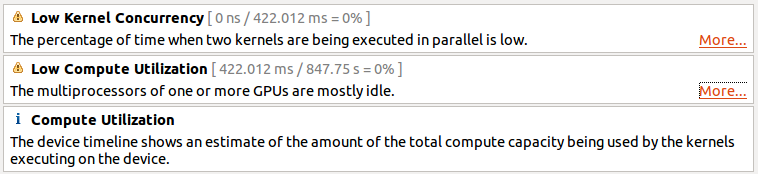
\includegraphics[width=.7\textwidth]{images/low-kernel-concurrency.png}
  \caption{nvidia Visual Profiler analysis indicates low kernel concurrency}
  \label{fig:first impl}
\end{figure}
